Thus, we observed that tau unbinding from the islands depends on the tau concentration in solution and suggests that the underpinning interactions are multivalent, which, indeed, can be expected due to the presence of four microtubule binding repeats (4R) in the 2N4R tau molecules. Precedent for this observation are, for example, the concentration-dependent unbinding rates of multivalent DNA-binding proteins15.

We can say that the high nucleation rate in the beginning hints at some regions having more affinity than others and link to \cite{siahaan2022microtubule}

\begin{figure}[h!tb]
\centering
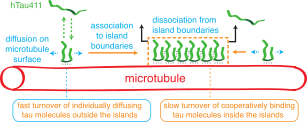
\includegraphics[scale=1]{Figures/tau8.png}
\caption[Schematic representation of island formation.]{
\textbf{Schematic representation of island formation.} Tau molecules bind and unbind with high rates to microtubules, on which they diffuse (fast turnover). When encountering an island (dashed orange box), tau molecules cooperatively associate with the island at its boundaries, rendering the tau molecules stationary, decreasing their unbinding rate (slow turnover), and causing the island to grow in size laterally. Tau molecules from solution can only bind to the inside of an island via displacement of an island-associated tau molecule, resulting in the observed concentration-dependent turnover of tau inside islands. After removal of tau from solution, tau molecules dissociate from the island boundaries, making the island shrink in size laterally.
	}\label{tau8}
\end{figure}
Taken together we show that tau on microtubules can co-exist in two kinetically distinct phases, manifested in the reversible formation of cohesive islands, cooperatively compounded of stationary tau molecules with a low turn-over rate. These islands form in a pool of discretely binding, diffusible tau molecules with a high turn-over rate (Figure 7). At physiological concentrations the islands colocalize with a layer of high turn-over tau, which can obscure the position of the islands. Tau islands reversibly regulate the local accessibility of the microtubule surface, and thus locally control katanin severing and kinesin-1 mediated transport. The tau islands described in our study are fundamentally distinct from the patches of clustered tau reported earlier9, as islands form reversibly by growing from their boundaries, forming a uniform layer and shielding the entire accessible surface of microtubules.
Tau islands display a characteristic density (0.25 - 0.45 nm-1), which is similar to the value of complete coverage, estimated recently by cryo-electron microscopy (~0.43 nm-1), suggesting that islands are monolayers of tau as shown in the respective study21. Further increasing the concentration of tau in solution in our experiments resulted in an increase in the density of tau that rapidly turned over on the microtubule surface, obscuring the islands at physiological tau concentrations. A reason why this pool of tau was not captured by cryo-electron microscopy experiments could be the transiency of the interactions, which might be mediated by the C-termini of tubulin as suggested earlier4. Importantly, this phase of rapidly turning over tau molecules was not able to protect microtubules from katanin severing even at saturating densities at micromolar concentrations. By contrast, islands protected the microtubule from katanin at tau concentrations as low as 20 nM, showing that it is not the density of tau molecules, but the cohesion between the cooperatively binding tau molecules constituting the island, which protects the microtubules from degradation by katanin. 
Islands assemble and disassemble predominantly at their boundaries suggesting that the integrity of the islands depends on cooperativity between the constituting tau molecules. Tau is known to undergo liquid-liquid phase separation in solution which is underpinned by tau-tau interactions25. As tau-tau interaction on the microtubule have been reported earlier26, it seems plausible that tau-tau interactions also underpin the formation of islands. Alternatively, or additionally, cooperativity could depend on the local modification of the microtubule surface by tau binding, which translates along the microtubule lattice into adjacent binding sites, increasing the affinity of incoming tau molecules for these adjacent binding sites.	
How can kinesin-8 displace such cohesive tau islands? Tau molecules possess four microtubule-binding-repeats, which separately interact with one tubulin dimer each, occupying similar binding site as the kinesin motor domain21. While tau proteins are bound multivalently to the periodic surface of the microtubule, the four microtubule-binding-repeats of a tau molecule each bind and unbind individually. Importantly, kinesin-8 motors do not dissociate when the next binding site on the microtubule is not available. We hypothesize that this ability enables them to wait until, stochastically, the next binding site becomes available by transient tau repeat unbinding and, in this way, sequentially replace the four microtubule-binding-repeats. During this process the kinesins have to overcome just the affinity of a single microtubule-binding repeat, not the avidity of the whole tau molecule.
The ability of kinesin-8 motors to disassemble the islands suggests that the accessibility of the microtubule surface is governed by an interplay between the avidity of cooperatively binding tau molecules constituting the cohesive islands and affinity of other axonal MAPs. The human kinesin-8, Kif18A, is involved in regulating axonal microtubule dynamics17 and, like its S. cerevisiae orthologue Kip3, employed in the current study, was described in vitro as super-processive molecular motor19,27. Kif18A thus possesses the crucial property required for a molecular motor to displace tau islands and therefore might be involved in regulating the localization of tau in neurons, and reciprocally, might be regulated by tau islands, which, we showed, initiate traffic jam formation at their boundaries, and reduce the speed of the motors that enter the island-covered region. 
In summary, we show that tau on microtubules separates into the kinetically distinct phases over a broad range of conditions. Complementary work presented in Tan et al. confirms the existence of tau phase-separation on the microtubule surface and shows its significance for the regulation of cytoplasmic dynein and spastin, extending our results28. We hypothesize that the islands of stationary tau can tag specific regions on the microtubules, for example as a readout of differential post-translational modifications of tubulin, rendering the regions on the microtubule surface differentially accessible to other MAPs. Sorting of proteins associated with cytoskeletal filaments can be driven by reciprocal exclusion generated e.g. by geometrical constraints29 or localized binding of different intrinsically disordered proteins30. As tau is not the only disordered protein to have a propensity to undergo liquid-liquid phase separation, we hypothesize that other disordered proteins might be also be able to phase-separate on the microtubule surface, which could add another layer of MAP sorting and regulation on microtubules. It is intriguing to speculate that in neurodegenerative diseases, which involve the gradual dissociation of unstructured proteins from neuronal microtubules, diminished island assembly, triggered e.g. by hyperphosphorylation of tau, could be a cause for various downstream (patho-)physiological effects. 
